\documentclass[border=0pt]{standalone}
\usepackage{fontspec}
\setmainfont{Carlito}
\usepackage{unicode-math}
\setmathfont{Latin Modern Math}
\usepackage{xcolor}
\usepackage{booktabs}
\usepackage{tikz}
\usepackage{graphicx}

\definecolor{canvabg}{RGB}{246,244,241}
\definecolor{textDark}{RGB}{40,40,40}
\definecolor{textMute}{RGB}{125,120,113}
\definecolor{accent}{RGB}{18,125,108}
\definecolor{trough}{RGB}{160,55,50}
\definecolor{bridge}{RGB}{30,90,140}

\pagecolor{canvabg}

\providecommand{\Cref}[1]{}
\providecommand{\cref}[1]{}
\providecommand{\ab}[1]{#1}

\renewcommand{\arraystretch}{1.25}

\begin{document}
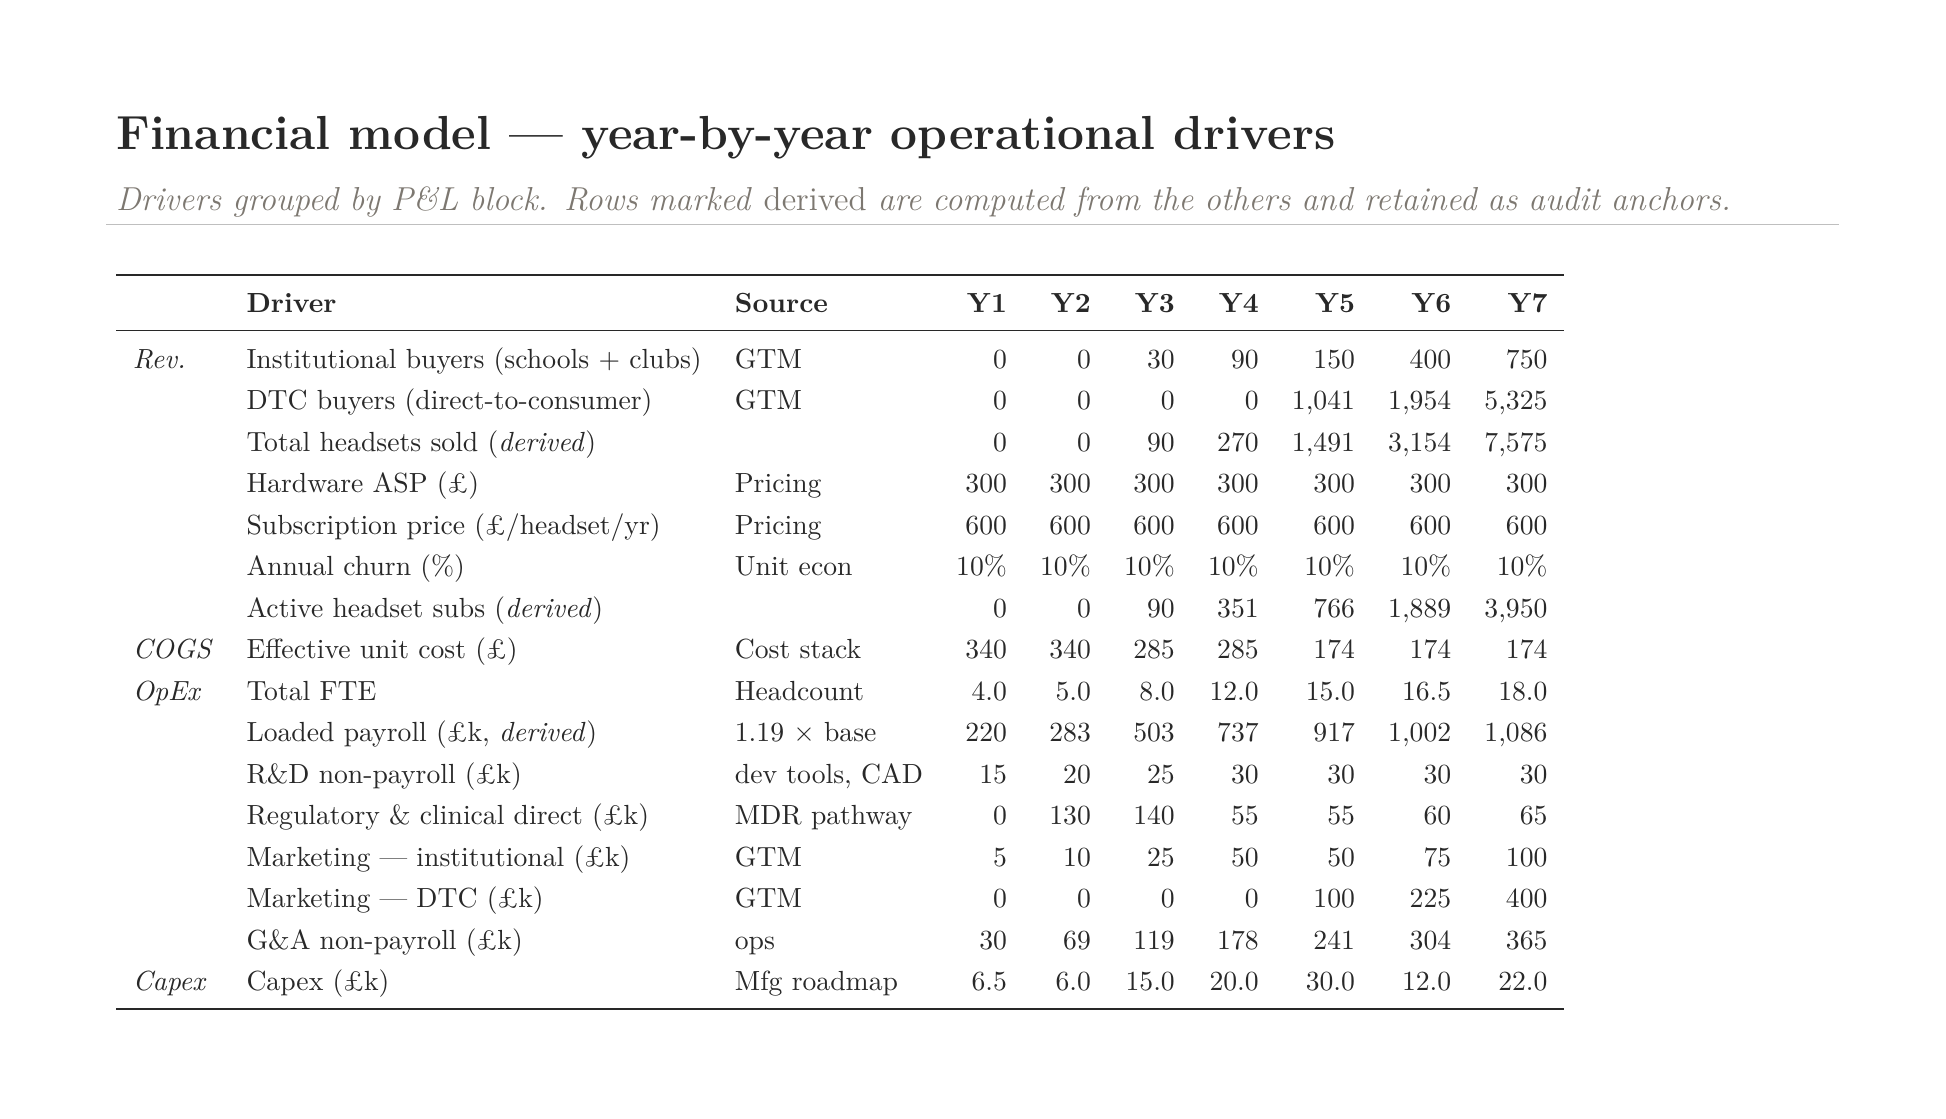
\begin{tikzpicture}[every node/.style={text=textDark}]
\useasboundingbox (0,0) rectangle (24, 13.5);

\node[anchor=north west, font=\bfseries\LARGE] at (1.0, 12.5)
    {Financial model — year-by-year operational drivers};
\node[anchor=north west, font=\itshape\large, text=textMute, text width=22cm]
    at (1.0, 11.6)
    {Drivers grouped by P\&L block. Rows marked \emph{derived} are computed
     from the others and retained as audit anchors.};

\draw[gray!50, line width=0.5pt] (1.0, 11.0) -- (23.0, 11.0);

\node[anchor=north west, font=\normalsize] at (1.0, 10.5) {%
\begin{tabular}{lllrrrrrrr}
    \toprule
     & \textbf{Driver} & \textbf{Source} & \textbf{Y1} & \textbf{Y2} & \textbf{Y3} & \textbf{Y4} & \textbf{Y5} & \textbf{Y6} & \textbf{Y7} \\
    \midrule
    \textit{Rev.} & Institutional buyers (schools + clubs) & GTM & 0 & 0 & 30 & 90 & 150 & 400 & 750 \\
     & DTC buyers (direct-to-consumer) & GTM & 0 & 0 & 0 & 0 & 1{,}041 & 1{,}954 & 5{,}325 \\
     & Total headsets sold (\emph{derived}) &  & 0 & 0 & 90 & 270 & 1{,}491 & 3{,}154 & 7{,}575 \\
     & Hardware ASP (\pounds) & Pricing & 300 & 300 & 300 & 300 & 300 & 300 & 300 \\
     & Subscription price (\pounds/headset/yr) & Pricing & 600 & 600 & 600 & 600 & 600 & 600 & 600 \\
     & Annual churn (\%) & Unit econ & 10\% & 10\% & 10\% & 10\% & 10\% & 10\% & 10\% \\
     & Active headset subs (\emph{derived}) &  & 0 & 0 & 90 & 351 & 766 & 1{,}889 & 3{,}950 \\
    \textit{COGS} & Effective unit cost (\pounds) & Cost stack & 340 & 340 & 285 & 285 & 174 & 174 & 174 \\
    \textit{OpEx} & Total FTE & Headcount & 4.0 & 5.0 & 8.0 & 12.0 & 15.0 & 16.5 & 18.0 \\
     & Loaded payroll (\pounds k, \emph{derived}) & 1.19 \texttimes{} base & 220 & 283 & 503 & 737 & 917 & 1{,}002 & 1{,}086 \\
     & R\&D non-payroll (\pounds k) & dev tools, CAD & 15 & 20 & 25 & 30 & 30 & 30 & 30 \\
     & Regulatory \& clinical direct (\pounds k) & MDR pathway & 0 & 130 & 140 & 55 & 55 & 60 & 65 \\
     & Marketing — institutional (\pounds k) & GTM & 5 & 10 & 25 & 50 & 50 & 75 & 100 \\
     & Marketing — DTC (\pounds k) & GTM & 0 & 0 & 0 & 0 & 100 & 225 & 400 \\
     & G\&A non-payroll (\pounds k) & ops & 30 & 69 & 119 & 178 & 241 & 304 & 365 \\
    \textit{Capex} & Capex (\pounds k) & Mfg roadmap & 6.5 & 6.0 & 15.0 & 20.0 & 30.0 & 12.0 & 22.0 \\
    \bottomrule
\end{tabular}
};

\end{tikzpicture}
\end{document}
